%!TEX root = ../thesis.tex

\chapter{System Overview}
\label{sec:systemoverview}

The system consists of two major parts.
First, the back end consisting of the local infrastructure monitoring and controlling temperatures and persisting this data on an accessible web server.
Second, the mobile application offering a user friendly interface to configure and interact with the system.
See Figure~\ref{fig:system_overview} for a graphical overview.

\begin{figure}[h]
\begin{center}
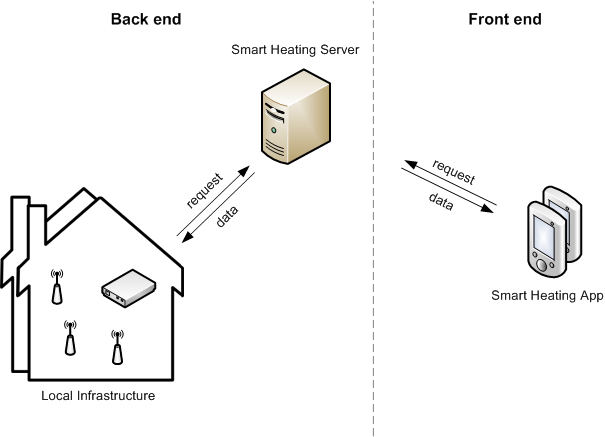
\includegraphics[width=0.9\textwidth]{images/SystemOverview.png}
\end{center}
\caption{
	System overview showing the infrastructure part and the mobile application part.
	The local infrastructure is required for each residence and a residence can be controlled using one or multiple mobile applications.
	The server is required only once and stores the information about all residences.
	}
\label{fig:system_overview}
\end{figure}

The infrastructure part consists of the local residential deployment and the server.
Within the residence a small computer system is installed which serves as a communication gateway to the distributed low-power thermostats.
On the remote side is the server acting as the central entity to collect and store the accumulated sensor data and organizational data.
Both are explained in Chapter~\ref{sec:infrastructure}.

The mobile application part \dots
\todo[inline]{SAMUEL: Mobile App text}

\section{Architecture}

The smart heating system is implemented using a server-client model.
% Willi: What does that mean? Describe briefly (in one or two sentences) which functionality is implemented where
The smart heating server hosts a web service acting as an API to provide access to the shared resources.
The local communication gateway uses this API to query the residence configuration and persist the collected measurements.
%The server handles requests from its clients to retrieve or store data.
%A local communication gateway uses this API in two ways.
%First, it queries residence information such as the associated thermostats and the heating schedule.
%Second, it persists the measured temperature data on the server to make it available to other clients.
Complementary, there is the mobile application also acting as a client.
It provides and updates the residence configuration and retrieves sensor data.
%This data is shared to the web server and required sensor data is queried conversely.
%The web server and the local infrastructures form the back end of the whole system whereas the mobile applications running on smart phones represent the front end.
%See Figure~\ref{fig:systemoverview_architecture} for a visual representation.


%\begin{figure}[h]
%	\begin{center}
%		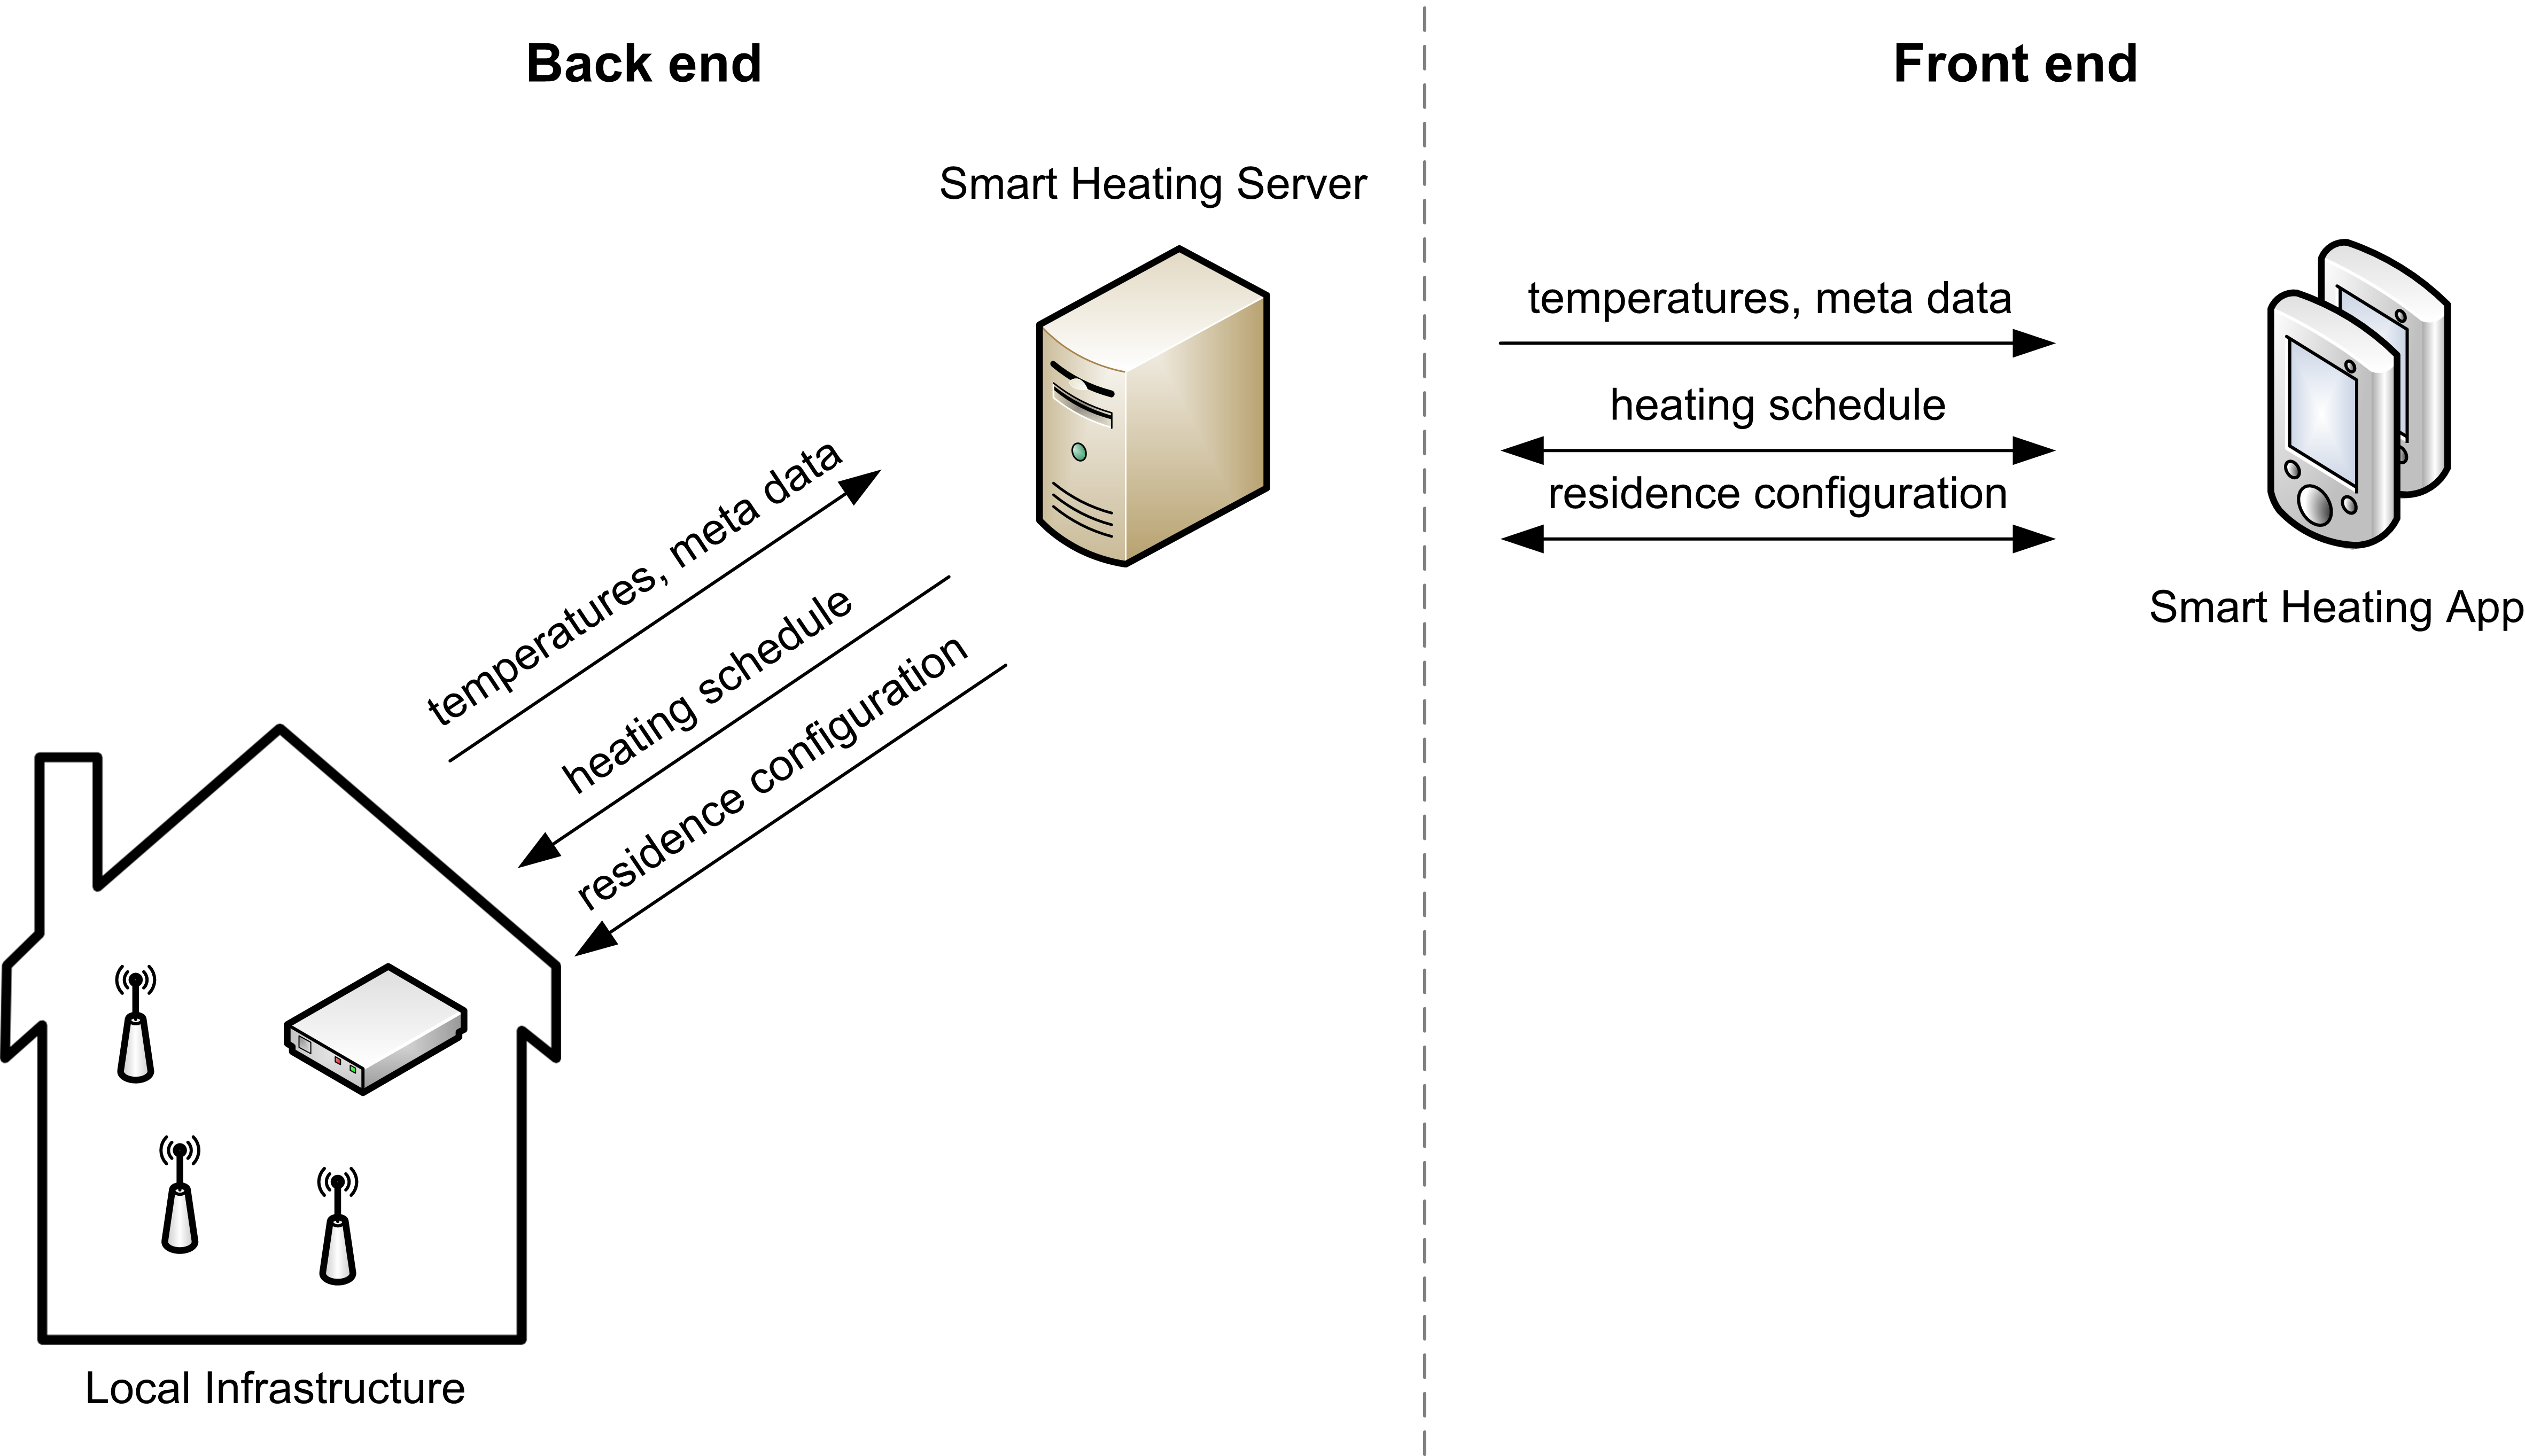
\includegraphics[width=0.95\textwidth]{images/SystemArchitecture.png}
%	\end{center}
%	\caption{Back end and front end depicting the communication between the server and its clients.}
%	\label{fig:systemoverview_architecture}
%\end{figure}


\section{Models}
\label{sec:system_overview_models}

Throughout the project there is a shared system model describing the underlying entities. The system model depicts the physical objects and places that are used for data collection or organizational purposes. The following paragraphs describe the applied models and their associated design decisions.

\todo[inline]{
	The relationship between the entities could also be represented in a diagram. Think of visualising the use cases. These terms should match the ones in the use-case section.\\
	SAMUEL: Falls du hier was passendes in den use cases hast ;)
	}

\paragraph{Residence}

The fundamental unit of each deployment is the residence. Each residence corresponds to an installed local communication gateway. Further details are described in Section~\ref{sec:local_infrastructure}

\paragraph{User}

Each residence can contain multiple users. A user is associated to exactly one residence and is identified by his smart phone IMEI. This design decision simplifies the system design and especially the user authentication. It also prevents a user from using the same identity when accessing the system from multiple smart phones.

\paragraph{Room and Thermostat}
A residence is divided in rooms where each room can contain several thermostats. A room is a simple organizational approach to group multiple thermostats into a single unit.
%Eine Residence ist unterteilt in Räume wobei jeder Raum mehrere Thermostat enthalten kann.

\paragraph{Heating Table}

Each thermostat has an associated temperature schedule called heating table.
The heating table is responsible for mapping each day and time in a week to a target temperature. The heating table is a periodic schedule repeating each week.
This design decision was chosen for infrastructure simplicity as well as to reduce usability complexity.

\paragraph{Meta Entries}

Meta entries persist time depending meta information about thermostats. A meta entry consists of the received signal strength, up-time, battery level and an associated timestamp. This data can be used to identify issues regarding the thermostat devices such as wireless connection problems or drained batteries.